%% ----------------------------------------------------------------------------
% BIWI SA/MA thesis template
%
% Created 09/29/2006 by Andreas Ess
% Extended 13/02/2009 by Jan Lesniak - jlesniak@vision.ee.ethz.ch
%% ----------------------------------------------------------------------------


\chapter{Introduction}
Image segmentation is a central task in biomedical image processing and image analysis. It can be used for detecting various diseases, shape diagnosis etc. The dataset which we are trying to segment is electron microscopic (EM) images of liver tissue. The dataset consists of a 3D stack of 2D slices of liver tissue as shown in figure 1.1. The image stack was generated at EMEZ (Electron Microscopy ETH Zürich) autonomously by iter-
atively cutting off a slice of the sample and scanning the cut face. With very little
interaction, the apparatus produced an output of 458 slices in 20 hours. The aim of this thesis is to compare and analyze different segmentaion methods to segment objects in histology images. In the following section, we describe the difficulties faced in segmentation of the histology images and give an overview of the methods used for segmentation. 

\begin{figure}[h!] \label{fig:3dstack}
\centering
 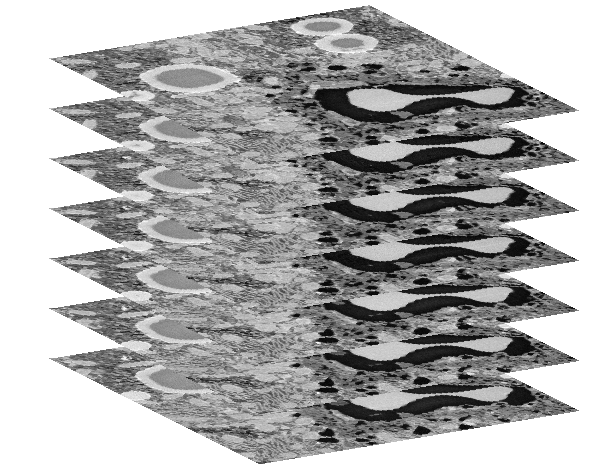
\includegraphics[width=0.8\linewidth]{figures/3d_stack.png}
\caption{A 3D image stack of liver tissue, output from a scanning electron microscope.
The stacks contains 458 2D images with a resolution of 1890x1952 pixel each.}
\end{figure}



\section{Segmentation of Histology Images}
The image segmentation is the process of partitioning a digital image into multiple segments. More precisely, image segmentation is the process of assigning a label to each pixel in an image such that pixels with the same label belong to same object. The main difficulty arises in assigning the labels to the pixels at the boundaries, which are difficult to discriminate from the surrounding pixels. The task of segmentaion in classical computer vision scenario, mainly consists of segmenting well defined objects  such as chairs, faces. Due to this reason, the ground truth annotated masks for training can be generated with comparative ease. As opposed to classical scenario, the objects segmented in the histology images do not have known shapes and are not well defined. This difficulty can be obsereved in figure 1.2 where it can be seen that the shape of the nuclei is not well defined and even unknown to experts. In contrast to classical scenario, segmenting histology image data faces the following challenges:
\begin{itemize}
\item High variability between image data: The images to be segmented may be entirely different i.e. having fixed objects as in liver tissue or having layers to segments as in neuron tissue. The objects to be segmented may differ completely from being smooth (round vesicles) to branched (neurons). We can observe few objects of interest in figure 1.2.
\item High variability between objects to segment: The object of interest, that the experts try to segment, may vary significantly in shape, size, and texture.
\item High variability between goals: Even for a single image, the goal of the segmentation can be totally different. The images annotated for one object can not be used again for training purpose.
\end{itemize}

\begin{figure}[h!] \label{fig:vesicles}
\centering
 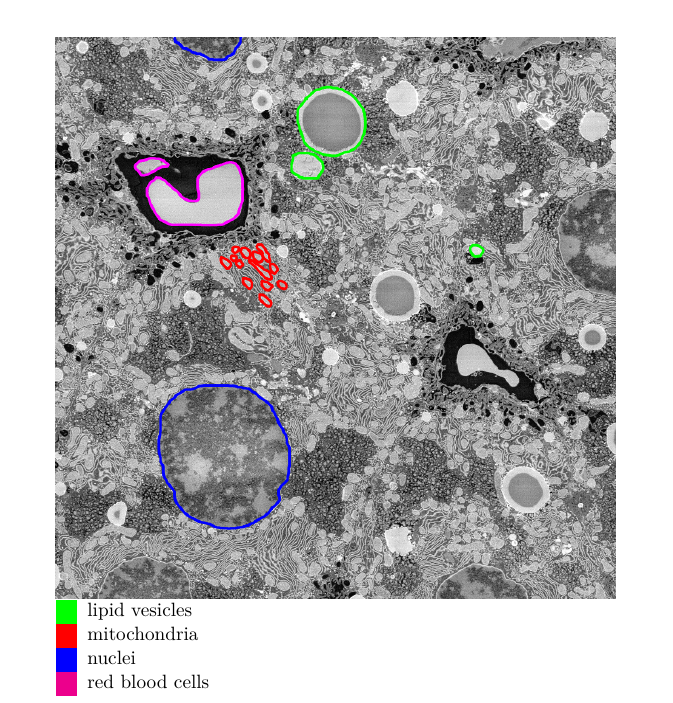
\includegraphics[width=0.8\linewidth]{figures/vesicles.png}
\caption{EM image of the liver tissue showing different objects of interest to experts.}
\end{figure}

\begin{figure}[h!] \label{fig:2dslice}
\centering
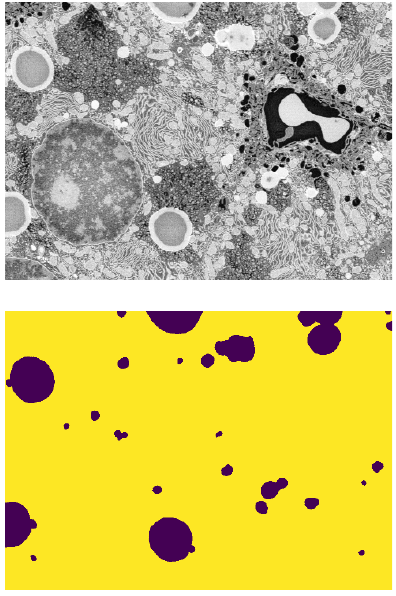
\includegraphics[width=0.65\linewidth,angle=90]{figures/ex_slice.png}
\caption{An example of the 2D slice and its segmentation mask showing vesicles as Foreground. Foreground: Purple, Background: Yellow}
\end{figure}


These characteristics of the histology images make it extremely difficult to fully annotate the objects and, becomes an extremely time-consuming task for experts. In this thesis, the focus is to segment vesicles in EM images of liver tissue (objects shown with green boundary in figure 2). The figure 1.3 shows a segmentation mask containing annotations for all vesicles in the cropped part of a slice. We can realize the difficulty in annotating multiple vesicles of undefined shapes and sizes. Most of the vesicles in figure 1.3 are of round shape but a few can be observed of having irregular shape. We can also observe the huge variation in size of objects, making it difficult to recognize and even cumbersome to annotate. In addition to this intrinsic, the experts are uncertain about the existence of vesicles or about the shape, in certain parts of images due to similarity in appearance or shape to other objtects. This uncertainty is shown in figure 1.4, where the differences (bounded by red rectangles) can be observed in manually annotated segmentation mask of the same image done by different experts. Moreover, sometimes there are differences in the masks for the same slice, annotated by the same expert at different times (shown in figure 1.5). The figure 1.5 shows difficulty in annotaion of vesicles due to not so well defined shapes and size of microscopic objects in microscopic images. This uncertainty has been analyzed a lot in literature and researchers have tried to come up with different methods to generate a ground truth mask from these multiple annotations by experts. The literature provide options of using either STAPLE \cite{staple} algorithm, or union, or majority voting to derive reference mask. The reference mask derived for one slice using the STAPLE and the union method is shown in figure 1.6. The choice of method differs for different tasks and varies according to the goal of the task. In this thesis, we make use of reference masks generated by the STAPLE algorithm and the union method to evaluate our approaches for the task of segmentation.

\begin{figure}[h!] \label{fig:diffexperts}
 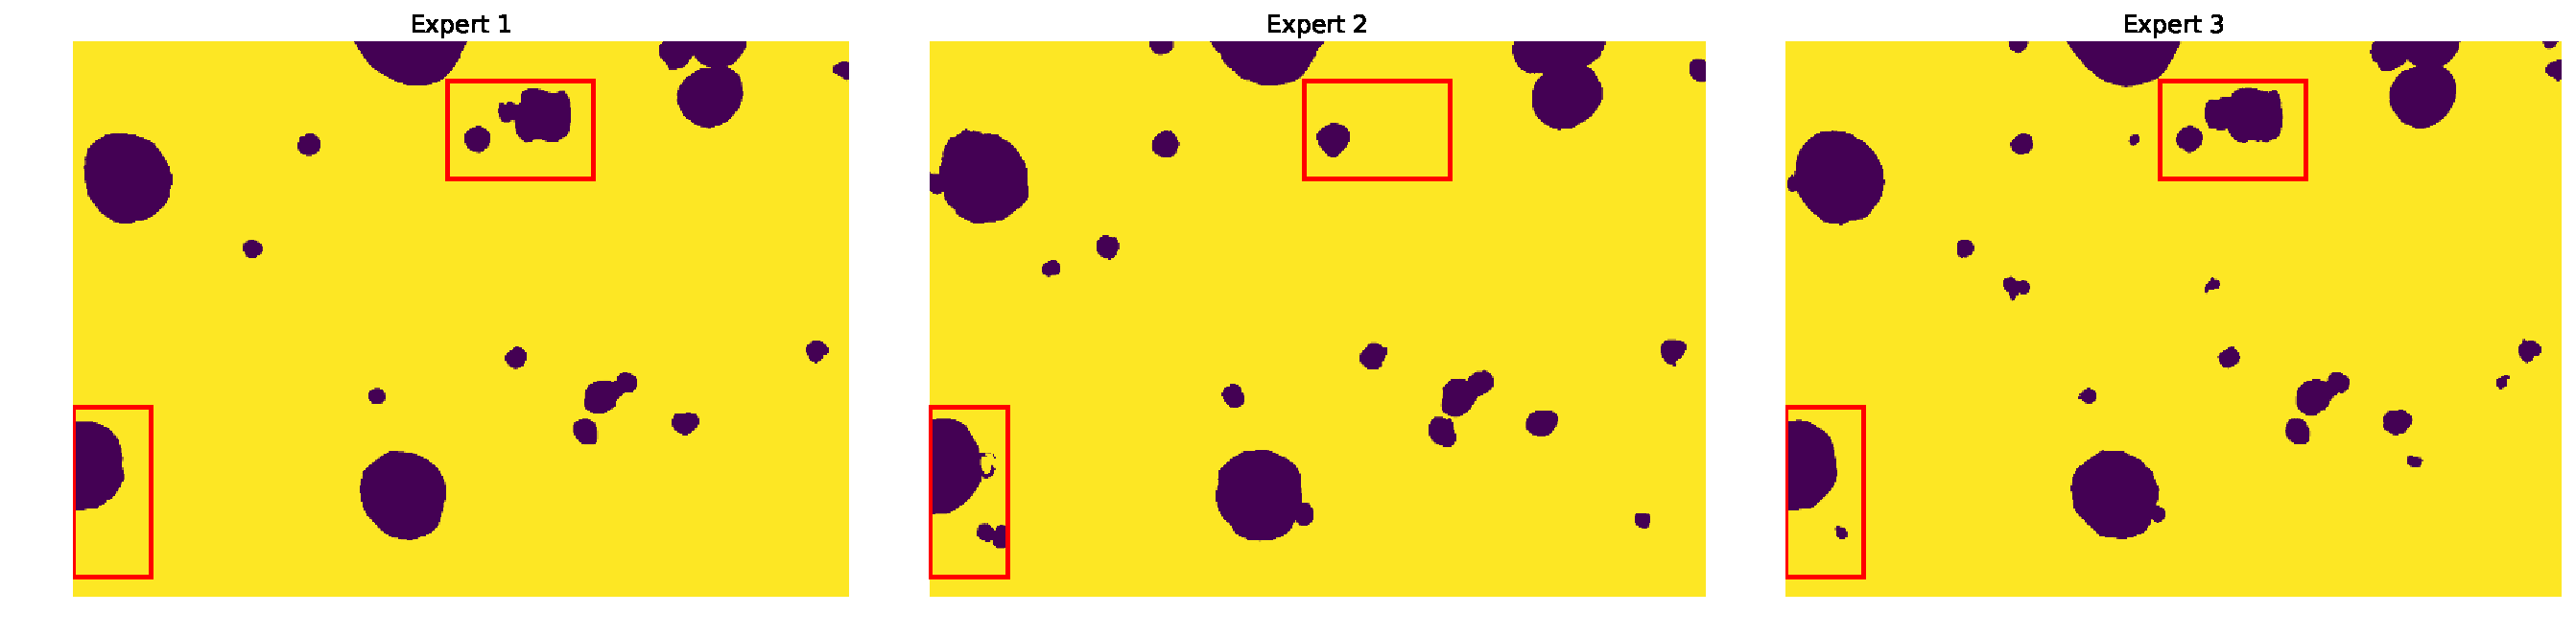
\includegraphics[width=1.0\linewidth]{figures/different_expert.pdf}
\caption{Segmentation mask for a slice annotated by different experts. The part of the mask bounded by red rectangles shows some of major differences.}
\end{figure}

\begin{figure}[h!] \label{fig:diffexperts}
  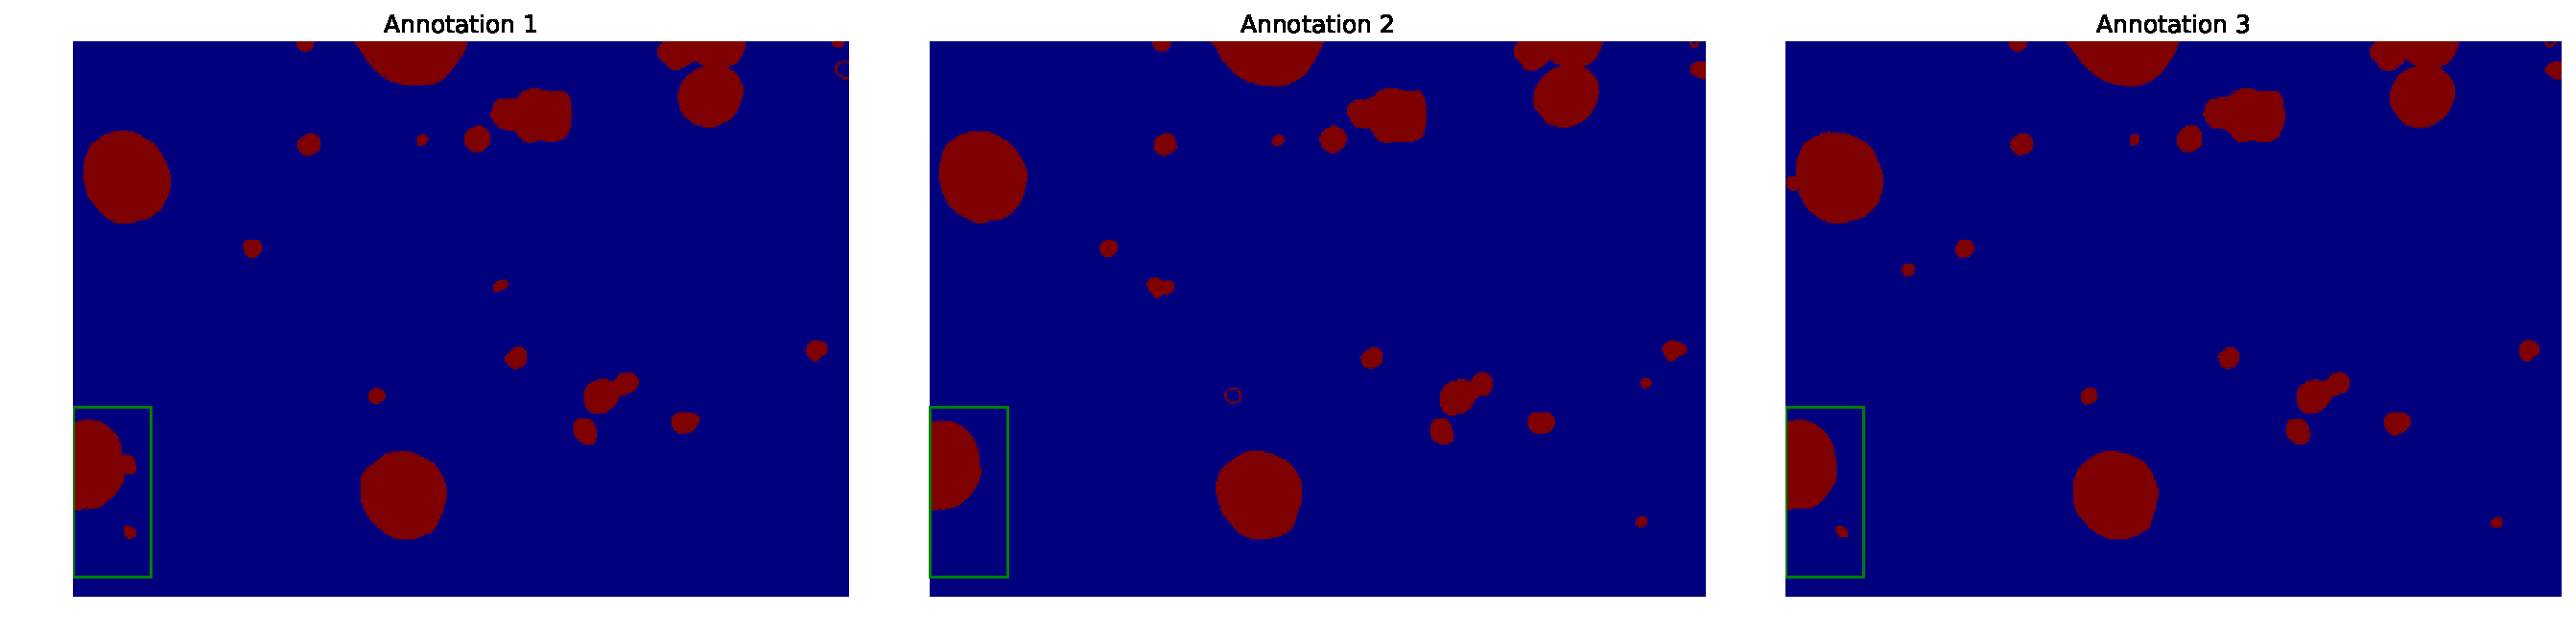
\includegraphics[width=1.0\linewidth]{figures/same_expert.pdf}
\caption{Segmentation mask for a slice annotated by same expert at different times.The part of the mask bounded by red rectangles shows some of major differences.}
\end{figure}

\begin{figure}[h!] \label{fig:ref}
\centering
 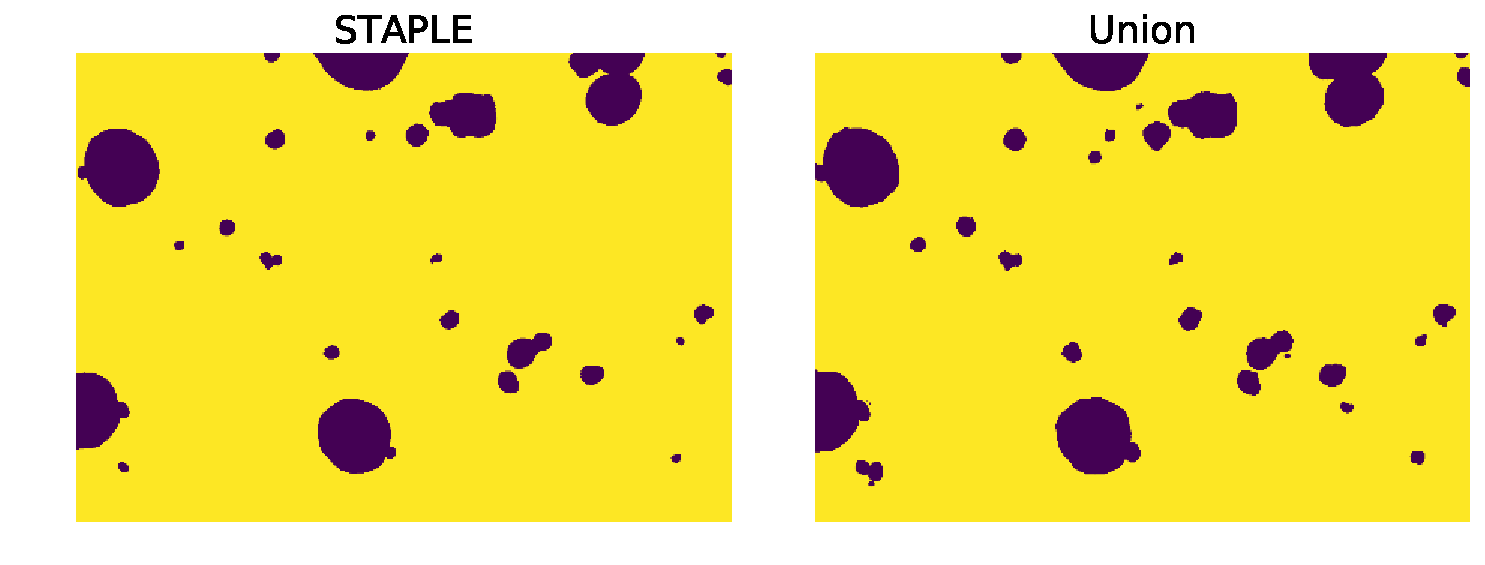
\includegraphics[width=0.7\linewidth]{figures/staple.pdf}
\caption{Grounth truth segmentation mask derived from multiple annotaions using 2 different methods (STAPLE and union).}
\end{figure}


\section{Focus of this thesis}
The focus of this thesis is to explore and analyze performance and limitations of two different methods, convolutional neural networks (CNN) and random forests (RF) to solve task of segmenting vesicles in 3D microscopic images of liver tissue. As we observed difficulty of obtaining significant amount of ground truth segmentation masks in previous section, we wanted to analyse the performance of these two approaches with variation of amount of training data. Initially, we tried CNNs using fully annotated segmentaion mask to obtain a benchmark for performance. Nowadays, it is common to train deep convolutional neural networks (DNN) using transfer learning to compensate for the scarce training data. We decided to choose a network pre-trained for segmentation task and fine-tune it for our problem. We chose a pre-trained network explained in Caelles \cite{osvos}. This paper describes a network, termed as \textbf{OSVOS}, which is designed for tackling the task of \textbf{semi-supervised} video object segmentation, i.e., segment an object in a video, given fully annotated mask of the object in the first frame. This task can be considered to be similar to segmenting objects in a 3D stack of slices. We tried to fine-tune the network using limited number of segmentation masks with fully annotated objects and obseved the variation in performance with increasing amount of training data (number of slices). The details of this approach and experiment are described in chapter 2.  \par
The use of pre-trained networks makes it possible to use DNNs even with small amount of training data. But still to train the DNNs, we need to provide the segmentation masks with fully annotated objects of interest for all training images. This comes out to be a tedious and difficult task for our problem as explained in previous section. In addition, the presence of multiple objects of different shape and sizes makes it even more difficult and time-consuming. Imagine 1000 cells in a 2D slice and possibility to manually annotate all these cells of undefined shapes! This leaves us with the option of annotating few objects and train networks using either cropped images or treating rest of image as background. Or we can use semi-supervised learning using partial annotations. In literature, we can find various methods to use these partial annotations to classify each pixel as foreground or background. We made use of Random Forests as described by Santner \cite{santner:2009} or Eugster \cite{dominic} for segmenting objects in images using partial annotations. In this thesis, the main focus was to discover the effect of annotation budget i.e. the number of pixels to annotate on the accuracy achieved. \par

The RFs learn pixel level information and are uncertain for the maximum of pixels i.e. the probability of foreground learned is not binary but lies between 0 and 1. The simple approach is to use thresholding to generate binary segmentation mask. In literature, different approaches can be found to use prior information to compensate for training data and for the uncertainty of estimators. The most common is to use Conditional random fields (CRFs) to regularize the probability mask learned from RFs. We solved this problem using a prior in \textbf{Bayesian framework} using Total Variation (TV) similar to method described in thesis by Eugster \cite{dominic}. In thesis of Eugster \cite{dominic}, they tried to learn likelihood using Random forests and implemented prior as an isotropic total variation (TV). They used a non-linear cost function to formulate likelihood from probabilities learned from Random forests. Instead of using a non-linear function to use probabilities, Santner \cite{santner:2009} uses a linear function to derive an energy minimization problem using probability mask obtained from RFs. This motivated us to analyze and compare these different cost functions and observe the advantage of using these cost functions in different scenarios. \par

In summary, we use a Bayesian approach with RF to parametrize likelihood and isotropic TV as prior to predict segmentation mask for a given image. This gives us chance to generate fully annotated segmentation masks and train CNN to obtain better accuracy. The common problem for use of prior is the choice of appropriate scaling to couple likelihood and prior costs. Ranftl \cite{ranftl:2014} coupled the prior cost function with the likelihood cost function obtained from CNN. They optimized the final loss function to obtain optimal values for network parameters (weights and biases) and regularization parameter. Riegler \cite{riegler:2016} \cite{riegler1:2016} proposed a method to implement TV as specialized layers in CNN and trained the complete model, CNN + TV, together. This motivated us to replace RF with CNN and try to fine-tune pre-trained fully convolutional network from partial annotations. We were able to restructure cross-entropy loss function of the pre-trained network to compute loss for partial annotations. We trained the CNNs using different annotation budgets and did a comparative analysis between results obtained for CNN and RF using different annotation budgets.

\section{Thesis Organization}
The thesis is divided mainly into two sections: segmentation using fully annotated objects and segmentation using partial annotations. The segmentation using full annotations is described in Section 2. The latter method is described in Section 3. In section 3.1, we describe the improvement in segmentation mask using RF for increased labeling effort. We introduce the use of prior and variational methods in section 3.2. In section 3.3, we introduce use of CNNs to learn from partial annotations. Finally, in the last section, we conclude this thesis and lay out future work that can be done.


